\subsection{User Interfaces}
\label{subsect:User Interfaces}
	The following mockups are an overall representation of the look of the app and the website in their first release.
	\subsubsection{Login}
	\begin{figure}[H]
	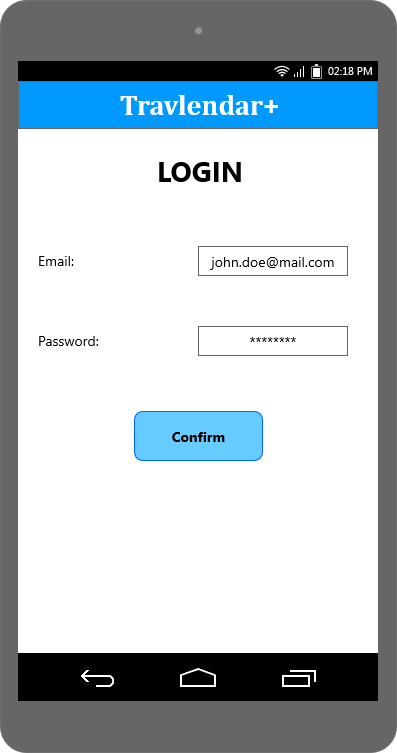
\includegraphics[scale=0.35]{mockup/app/Start/02-Login}
	\vspace{2.5cm}
	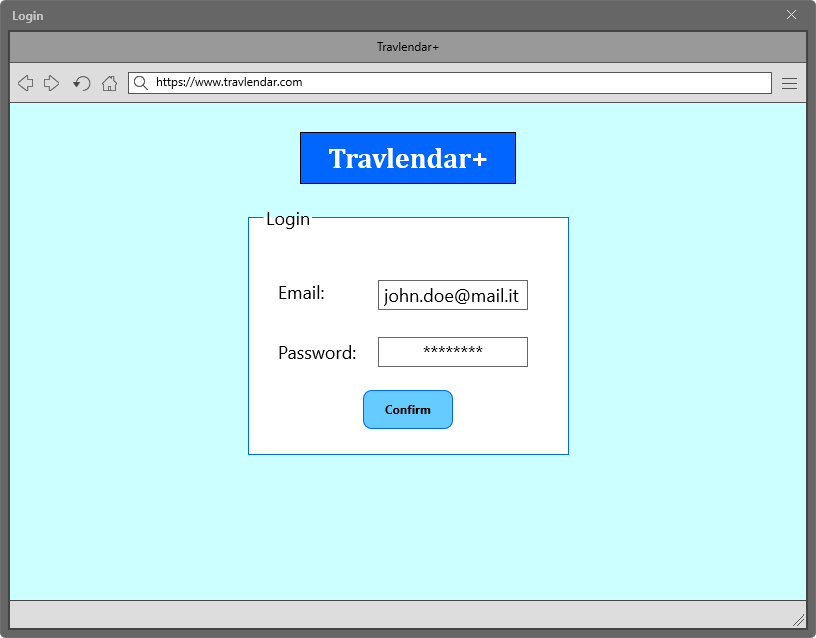
\includegraphics[scale=0.35]{mockup/web/01-Login}
	\centering 
	\end{figure}
	
	\subsubsection{Calendar and Map}
	\begin{figure}[H]
	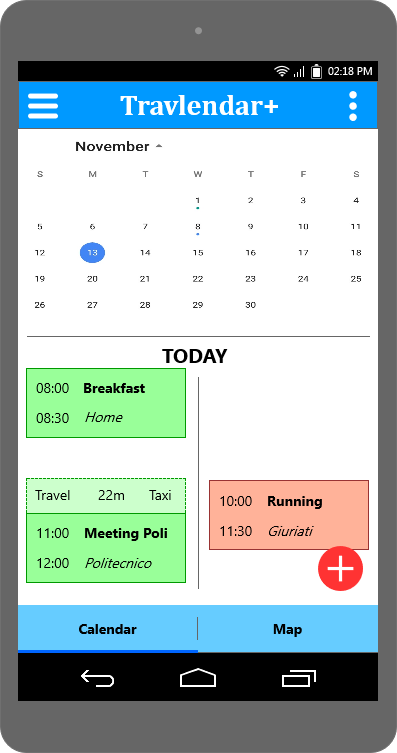
\includegraphics[scale=0.35]{mockup/app//Calendar/00-Calendar}
	\hspace{2.5cm}
	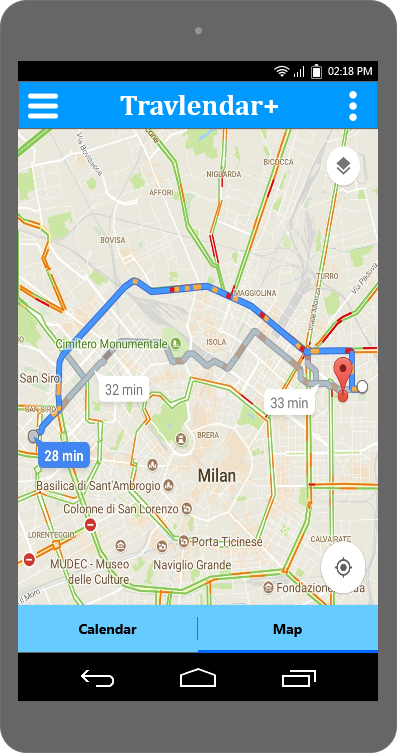
\includegraphics[scale=0.35]{mockup/app/04-Map}
	\centering 
	\end{figure}
	
	\subsubsection{Schedule and Event Creation}
	\begin{figure}[H]
	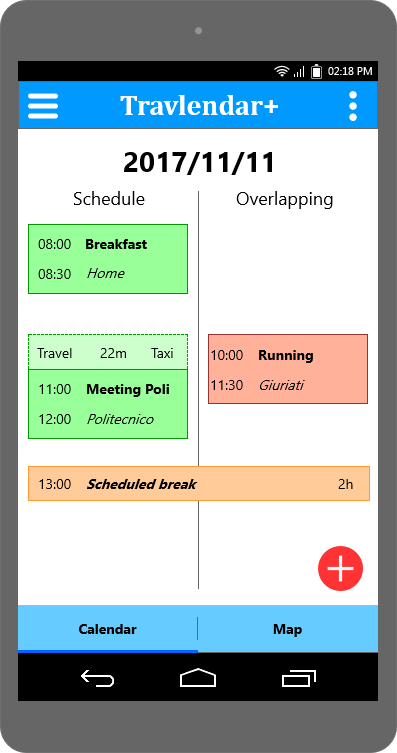
\includegraphics[scale=0.35]{mockup/app/Calendar/Schedule/00-Schedule}
	\hspace{2.5cm}
	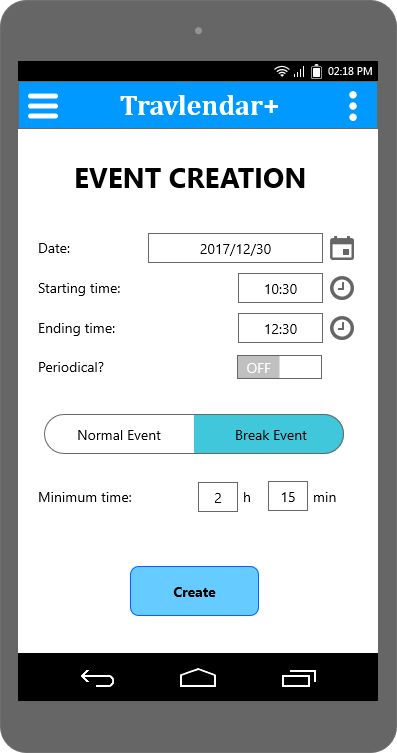
\includegraphics[scale=0.35]{mockup/app/Calendar/Create_Event/02-Create_Break_Event}
	\centering 
	\end{figure}
	
	\subsubsection{My Tickets and Preferences}
	\begin{figure}[H]
	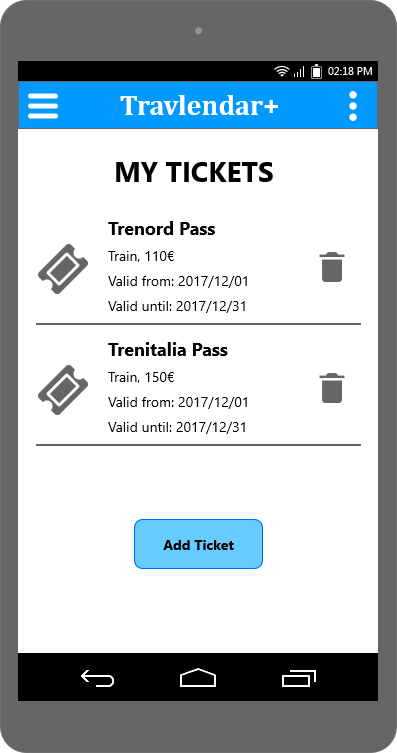
\includegraphics[scale=0.4]{mockup/app/My_Tickets/00-My_Tickets}
	\hspace{2.5cm}
	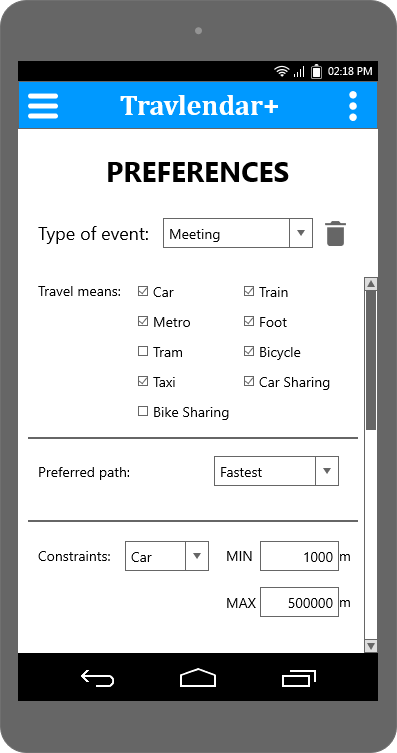
\includegraphics[scale=0.4]{mockup/app/06-Preferences}
	\centering 
	\end{figure}
	
	\subsubsection{Web View}
	\begin{figure}[H]
	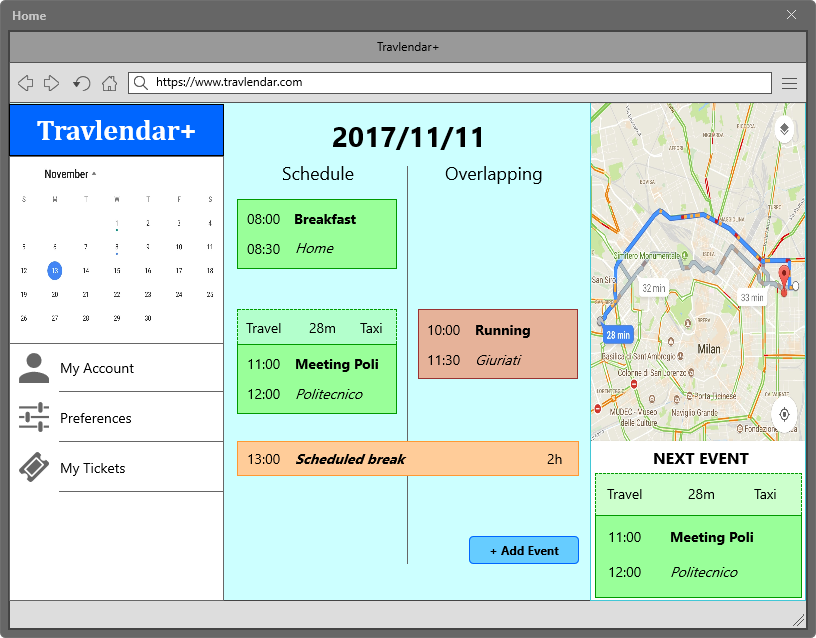
\includegraphics[scale=0.4]{mockup/web/02-Home}
	\centering
	\end{figure}
	
\newpage
\subsection{Hardware Interfaces}
\label{subsect:Hardware Interfaces}
	The mobile app is supported on:
	\begin{itemize}
		\item Android 6.0 and superior;
		\item iOS 8 and superior;
	\end{itemize}
	To utilize the mobile app, the phone must be able to connect to the Internet and have a working GPS sensor to identify its position. \\ \\
	The web app is supported on these browsers:
	\begin{itemize}
		\item Google Chrome;
		\item Mozilla Firefox;
		\item Microsoft Edge;
		\item Safari;
	\end{itemize}
	Other browsers may be utilized to access the web app, but full compatibility is not guaranteed.
\subsection{Software Interfaces}
\label{subsect:Software Interfaces}
	This system implements Google Maps APIs to calculate the optimal travel path to reach a destination. \\
	Interaction with external websites of travel means providers is required in order to allow the user to buy tickets. \\
	External weather APIs will be used to gather weather forecast data in order to propose travels taking into account the weather in the computation process. \\
	The system implements Google Transit APIs in order to use GTFS and GTFS-realtime feeds to improve path computations when public travel means are involved.
	The system back-end (server side) will be implemented using Java EE 8 and we'll use MySQL 5.7 as DBMS.
	
	
\subsection{Communication Interfaces}
\label{subsect:Communication Interfaces}
	During the registration phase, the system will automatically send an email to the email address inserted by the user. \\
	This email will contain a recap of the data inserted by the user during the registration, along with a linked URL address that needs to be opened by the user in order to verify that that email is currently valid and active.
	The client will communicate with HTTP protocol by using TCP (default port 443).